\chapter{The Theory of PRex Experiment(~20)}

\begin{itemize}
    \item history of the nuclear structure
    \item scatter is used for nuclear structure probe, charge radius 
    \item neutron charges 0, poorly measured
    \item historical measurement 
    \item parity violation measurement of the neutron density
\end{itemize}

PRex experiment measures the neutron skin thickness with parity violation asymmetry. This chapter will introduce the theoretical aspect of the experiment: weak interaction, weak interaction form factor, APV, and neutron skin thickness.

The RMS radius of the  neutron distribution in a heavy nucleus  $R_N$ provides an important test of nuclear theory. Furthermore,   $R_N$ is used in the determination of  the density dependence of symmetry energy of neutron-rich matter; this dependence is an  essential input in   neutron star structure, heavy iron collision, and atomic parity violation experiment calculations. In the past hadron scattering experiments with pion, proton or anti-proton beams have been used to determine the neutron radii of heavy nuclei. However, these measurements suffer from uncertainties associated with the probe particle and the target nucleus. Electron scattering provides a model-independent probe of nuclear radii.  However, in electron scattering, the measurement of neutron distribution in a nucleus  is much harder than the measurement of the proton distribution  since the neutron is uncharged. 

\section{charge radius measurement}
[to be optimized, maybe merge with the e-w interaction part]
The charge radius of nucleus can be measured by electron scattering. The cross-section of electrons scattered over charged particles by changing photons can be written as:

\begin{equation}
    \frac{d\sigma}{d\Omega} = \frac{e^4}{4\pi*s}|\frac{M^2}{q^2 - m^2_\gamma + i\epsilon}|^2
\end{equation}

Here in the equation,  e is the electron charge, $s = (k_1 + p_1)^2$ is the Mandelstam variable, $m_\gamma$ is the mass of the photon, and $\epsilon$ is a positive infinitesimal. 

In point-like particle approximation, the potential is the coulomb potential: 
\begin{equation}
    V(r) = \frac{e^2}{r}
\end{equation}

The scattering amplitude can be written as $f(q) = \frac{e^2}{q^2}$, here in the equation $q$ is the four-momentum transfer.

Put the equation in the Klein-Gordon formula, the cross-section can be written as:

\begin{equation}
     \frac{d\sigma}{d\Omega} = \frac{e^4}{4\pi*s}|\frac{M^2}{q^2 - m^2_\gamma + i\epsilon}|^2|f(q)|^2
\end{equation}

In the non-relativistic limit, $s \simeq 4M^2$ and $q^2 = \simeq 4M^2 \sin^2{\theta/2}$, 
\begin{equation}
    \frac{d\sigma}{d\Omega} = \frac{e^4}{4\pi*s} \frac{M^4}{q^4}|f(q)|^2
\end{equation}

\begin{equation}
    f(q) \simeq \frac{e^2}{q^2} - \frac{e^2\alpha}{2q^4}
\end{equation}

Here $\alpha = \frac{e^2}{4\pi}$ is the fine-struture constant:

The cross-section can be written as:
\begin{equation}
      \frac{d\sigma}{d\Omega_{Mott}} =   \frac{e^4}{4\pi*s} \frac{4M^2\sin^4{(\theta/2)}}{(E_1^2 - p_1^2\sin^2{\theta/2})^2}
\end{equation}

Where $E_1$ and $p_1$ are the energy and momentum of the incident electron. 


For no-point-link particles, the Charge distribution of nuclei is measured by electron scattering. The cross-section can be written as
\begin{equation}
    \frac{d\sigma}{d\Omega} = \frac{d\sigma}{d\Omega_{Mott}}|F_p(Q^2)|^2
\end{equation}

Here is the equation the first part $\frac{d\sigma}{d\Omega_{Mott}}$ is the Mott cross-section with describes the cross-section of electron scattering over a point-like charged particles. The second part is the form factor of the charged particle which contains the structure information of the particle. 


\begin{equation}
    F_n(Q^2) = \frac{1}{4\pi}\int{j_0(qr)\rho_n(r)}d^3r
\end{equation}

In low $Q^2$ approximation, the form factor can be written as:
\begin{equation}
    F(Q^2) = \int{(1-i\Vec{Q}\Vec{r} - \frac{1}{2}(\Vec{Q}\Vec{r})^2)\rho(\Vec{r})}d^3r = Q_e - \frac{1}{6}Q^2<r^2> + ...
\end{equation}

At low four-momentum transfer approximation, the charge radius can be written as

\begin{equation}
    <r^2> = -6\hbar^2\frac{dF(Q^2)}{Q^2}|_{Q^2\simeq0}
\end{equation}

Through electron scattering, the charge radius of nuclei has been well measured. The charge radius of $^{208}Pb$ is measured as $R^{208}_{p} = 5.5012(13)fm$ with accuracy $0.02\%$\cite{ANGELI201369}.


\section{Theory background of the PRex experiment}

\subsection{concept}
\subsubsection{Parity}
In particle and nuclear physics, interactions are described by fundamental forces that are mediated by exchange particles, known as bosons. For a long time, it was believed that all fundamental interactions conserved parity, meaning that the laws of physics remained unchanged under spatial inversion. However, this assumption was challenged by the discovery of parity violation in weak interactions in the 1950s.

[add T.D. Lee and Yang's work]

The groundbreaking experiments by Chien-Shiung Wu and collaborators in 1957 demonstrated that weak interactions, responsible for processes such as beta decay, do not conserve parity. This discovery led to the revised understanding that while electromagnetic and strong interactions conserve parity, weak interactions do not. The recognition of parity violation has had a profound impact on the development of the Standard Model of particle physics and continues to shape research in fundamental physics.

Parity plays a significant role in the classification and understanding of particle and nuclear states. In particular, the determination of parity quantum numbers and their conservation (or violation) in various physical processes has provided important insights into the nature of interactions and symmetries.
[change needed, add parity plot]

\subsubsection{spin (to be improved)}

Spin is an intrinsic form of angular momentum carried by elementary particles. Spin obeys the principles of quantum mechanics, meaning it is quantized and can only take certain discrete values. The magnitude of spin for a particle is fixed and is usually represented by a non-negative integer or half-integer multiples of ħ (reduced Planck's constant). The z-component of spin (the component along an arbitrarily chosen direction, conventionally taken as the z-axis), however, can take values from -s to +s in steps of one, where s is the spin quantum number of the particle.

Fermions, which include particles like electrons, protons, and neutrons, are particles with half-integer spin (e.g., spin 1/2 for electrons and quarks). Their spin-statistics relation enforces the Pauli exclusion principle, which states that no two fermions can exist in the exact same quantum state simultaneously. This principle underpins the structure of atoms and hence much of chemistry and solid-state physics.

Bosons, on the other hand, are particles with integer spin, such as the photon (spin 1), the mediator of electromagnetic interactions, and the Higgs boson (spin 0). Multiple bosons can occupy the same quantum state, leading to phenomena such as Bose-Einstein condensates.

Spin plays a fundamental role in the behavior and interactions of quantum systems. For instance, the alignment or anti-alignment of spins in a system can drastically affect its properties, leading to the creation of ferromagnetic or antiferromagnetic materials. Spin is also critical in determining the characteristics of quantum states and their transformations under particle exchange and parity operations.

In the context of particle interactions, the conservation of angular momentum, which includes both orbital and spin components, is a fundamental principle. The spin of a particle influences how it interacts with other particles and fields, most prominently in interactions mediated by the spin-dependent weak nuclear force.

It's crucial to reiterate that despite the terminology, spin does not imply that particles are physically "spinning". Rather, it is a quantum mechanical property that shares mathematical similarities with the concept of angular momentum in classical physics but doesn't have a direct classical analog.

\subsubsection{Helicity}

In quantum physics, helicity is a key property of elementary particles that represents the projection of a particle's spin along its momentum vector. Consider a particle with a spin vector S and momentum vector p. The helicity h of the particle is defined as the projection of spin $\Vec{s}$ onto the direction of its momentum $\Vec{p}$

\begin{equation}
    H = \Vec{s}\frac{\Vec{p}}{|\Vec{p}|}
\end{equation}

The sign of helicity determines whether the particle is classified as right-handed or left-handed. A particle is said to have right-handed (or positive) helicity if its spin vector points in the same direction as its momentum vector. Conversely, a particle has left-handed (or negative) helicity if its spin vector points in the opposite direction to its momentum vector. 

Helicity is not a Lorentz invariant quantity for massive particles. In other words, different observers moving at different velocities may measure different helicities for the same particle if that particle has mass. This is because the direction of the momentum vector can be reversed in another frame of reference, which would flip the helicity. For massless particles, however, such as photons, which always move at the speed of light, helicity is conserved and is indeed a Lorentz invariant quantity.


\begin{figure}
    \centering
    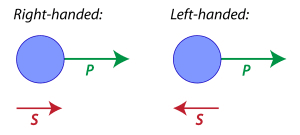
\includegraphics{images/chap2/rl_handed_particles.png}
    \caption{Left-handed and Right-handed Particles}
    \label{fig:left_right_handed_particles}
\end{figure}

\subsubsection{Chirality}

Chirality is a property of the particle's representation under the Poincaré group, and unlike helicity, it's a Lorentz-invariant quantity even for massive particles. In the Dirac equation, which describes spin-1/2 particles such as electrons and quarks, the chiral operator is represented by the $\gamma^5$ matrix which is defined as

\begin{equation}
 \gamma^5 = i\gamma^0\gamma^1\gamma^2\gamma^3 = \begin{pmatrix}
    0 & 0 & 1 & 0 \\
    0 & 0 & 0 & 1 \\
    1 & 0 & 0 & 0 \\
    0 & 1 & 0 & 0 \\
\end{pmatrix}   
\end{equation}

This operator has the property of commuting with the spatial part of the momentum operator but anticommuting with the Dirac Hamiltonian. Therefore, it serves as a tool to separate solutions of the Dirac equation into two distinct types, referred to as left-chiral and right-chiral solutions.


The chiral projection operators, denoted by $P_L$ (left-handed) and $P_R$ (right-handed), are defined in terms of the $\gamma^5$ matrix as follows:
\begin{center}
$P_L = \frac{1}{2}(1 - \gamma^5)$

$P_R = \frac{1}{2}(1 + \gamma^5)$    
\end{center}

These operators can be applied to a Dirac spinor to extract its left-chiral and right-chiral components. 

[to be optimized]

For massless particles, such as photons or neutrinos, chirality becomes a particularly meaningful concept because it corresponds exactly with helicity, the projection of spin onto the direction of motion. Because massless particles always move at the speed of light, no observer can outrun and "flip" the perceived helicity of the particle, making chirality a Lorentz invariant.

For massive particles, the situation is a bit more complex. Because they can move at different speeds, the helicity of a massive particle is not a Lorentz invariant quantity. This means that while a particle may appear left-handed in one frame of reference, it could appear right-handed in another. Despite this, the internal weak interactions of a particle still distinguish between its left-chiral and right-chiral components.

Chiral operator behave differently on left and right-handed fermions. On left-handed fermion: 

\begin{equation}
\begin{split}
    \gamma^5u_L &= \gamma^5P_Lu \\
     &= \gamma^5 \frac{1}{2}(1-\gamma^5)u \\
     &= \frac{1}{2}(\gamma^5 - (\gamma^5)^2)u \\
     &= - \frac{1}{2}(1 - \gamma^5)u \\
     &= - u_L
\end{split}
\end{equation}

for right-handed fermion, 
\begin{equation}
\begin{split}
\gamma^5u_R &= \gamma^5P_R \\
     &= \gamma^5 \frac{1}{2}(1+\gamma^5)u \\
     &= \frac{1}{2}(\gamma^5 + (\gamma^5)^2)u \\
     &= \frac{1}{2}(1 + \gamma^5)u \\
     &= u_R
\end{split}
\end{equation}

 [maximum  parity violation]
 
\subsection{Weak Current}

[...]

\section{Parity Violation Weak interaction}

\begin{itemize}
    \item electroweak interaction
    \item VA theory
    \item Parity Violation Weak interaction
    \item Parity Violating Asymmetry because of $\gamma$ and $Z^0$ exchange, $A_{pv} = \frac{\sigma_R - \sigma_L}{\sigma_R + \sigma_L}$
    \item weak form factor derived from the Parity Violating Asymmetry  $A_{pv}$
    \item neutron weak Form factor and n-structure
    \item get the density and the neutron skin thickness from PRex measurement
    \item the result from PRex-I experiment
    \item coulomb distortion
\end{itemize}

\subsection{weak interaction}
[into to 4 forces, and its mediators]

There are four fundamental forces governing the universe: strong force, weak force, electromagnetic force, and gravitational force. These forces vary in terms of their relative strengths and ranges. Among them, gravity is the most feeble, yet its influence is unbounded, extending infinitely. In contrast, the electromagnetic force, while also limitless in range, is significantly stronger than gravity. The strong and weak nuclear forces operate within a limited range, primarily influencing interactions at the subatomic level. Despite its name, the weak nuclear force is more potent than gravity but pales in comparison to both the electromagnetic force and the strong nuclear force. The strong force, as the name suggests, is the strongest of all four fundamental interactions.

The interaction of three of these fundamental forces—strong nuclear, weak nuclear, and electromagnetic—relies on the exchange of force-carrier particles, classified more broadly as bosons. These particles facilitate the transfer of discrete energy units between matter particles. Each fundamental force has a respective boson: the strong force is transmitted by gluons, photons carry the electromagnetic force, and W and Z bosons mediate the weak force. The corresponding boson for gravity, hypothetically, is the graviton, although its existence remains unconfirmed.

Unlike the photon and gluons, the weak force intermedia W and Z bosons are extremely heavy. 

\begin{equation}
    M_w = 80.40 \pm 0.03 GeV/c^2
\end{equation}

\begin{equation}
    M_z = 91.188 \pm 0.002 GeV/c^2
\end{equation}

\begin{table}[!h]
    \centering
    \begin{tabular}{c |c | c}
         Force  & Strength & Mediator \\ \hline
         Strong & 10  & Gluon \\ \hline
         Electromagnetic & $10^{-2}$ &  Photon \\ \hline
         Weak & $10^{-13}$ & W/Z boson \\ \hline
         Gravitational & $10^{-42}$ & Graviton \\ \hline
    \end{tabular}
    \caption{Fundamental Forces}
    \label{tab:my_label}
\end{table}


\subsection{Electroweak Interaction}

[need to optimize]
The electroweak interaction represents a profound unification in the world of particle physics. Initially proposed in the mid-20th century, it describes two of the four known fundamental forces - the weak nuclear force and the electromagnetic force - as distinct manifestations of a more fundamental electroweak force. This paradigm-shifting idea, posited by Sheldon Glashow, Abdus Salam, and Steven Weinberg, eventually earned them the Nobel Prize in Physics.

At its core, the electroweak theory is a quantum field theory (QFT), where particles are the quantized excitations of underlying fields, and their interactions are mediated by force-carrying particles. The electromagnetic force is mediated by photons, while the weak nuclear force is mediated by W and Z bosons.

To commence our exploration of the electroweak theory, let's first take a glance at quantum electrodynamics (QED), which describes the electromagnetic interaction. The Lagrangian density that encapsulates this interaction can be represented as:

\begin{equation}
\mathcal{L}_{\text{QED}} = \bar{\psi} (i\gamma ^\mu D _\mu - m)\psi - \frac{1}{4} F _{\mu \nu} F ^{\mu \nu}
\end{equation}

This QED Lagrangian can be extended to include the weak nuclear force, providing the foundation of the electroweak theory. In the electroweak model, the gauge group is $SU(2)_L x U(1)_Y$, symbolizing the weak isospin and weak hypercharge, respectively. The electroweak Lagrangian is given by:

\begin{equation}
\mathcal{L}_{\text{EW}} = \bar{\psi} (i\gamma ^\mu D _\mu - m)\psi - \frac{1}{4} W _{\mu \nu} W ^{\mu \nu} - \frac{1}{4} B _{\mu \nu} B ^{\mu \nu}
\end{equation}

Within this Lagrangian, the fermion mass term is not gauge invariant, leading us to the Higgs mechanism and the spontaneous symmetry breaking. The Higgs mechanism provides mass to the W and Z bosons, transforming them from massless gauge bosons into the massive particles observed in nature. 

This concept of electroweak unification and spontaneous symmetry breaking not only formulates the foundation of the Standard Model of particle physics but also imparts profound implications on our understanding of the fundamental structure of the universe. 


\subsection{Parity violation Electron Scattering}

[probably need to move to a better place]

The interaction of elestic elestron scattered over the nucleus involves electromagnetic interaction with exchange of photon $\gamma$ and weak interaction with the exchange of boson $Z^0$. The Feynman diagram can be written as:


The scattering amplitude matrix can be write as

\begin{equation}
    \mathcal{M} = \mathcal{M}_{\gamma} + \mathcal{M}_z
\end{equation}


Here in the equation $\mathcal{M}_{\sigma}$ is the scattering amplitude by exchange photon, and $\mathcal{M}_z$ is the scattering amplitude in weak interaction by exchange $Z$ mediator.  The cross-section of the elastic electrons over the nucleus can be written as, 

\begin{equation}
\begin{split}
        \frac{d\sigma}{d\Omega} &= \frac{dQ}{F} |  \mathcal{M}_z|^2 \\
        &= \frac{dQ}{F}|\mathcal{M}_{\gamma} + \mathcal{M}_z|^2 \\ 
        &= \frac{dQ}{F}(|\mathcal{M}_{\gamma}|^2 + 2*\mathcal{M}_{\gamma}\mathcal{M}_z + |\mathcal{M}_z|^2)
\end{split}
\end{equation}

Here in the equation, $F$ is the flux, and Q is the four-momentum transfer. The ratio of $|\mathcal{M}_{\gamma}|^2 : \mathcal{M}_{\gamma}\mathcal{M}_z : |\mathcal{M}_z|^2 = 1 : 10^{-4} : 10^{-9}$. The electromagnetic cross-section part is much larger than that of the weak interactions. Direct measurement would be impossible because of measurement errors. 


Elastic electron scattering has provided the most accurate and detailed picture of the distribution of protons in the atomic nucleus. As we can see from the above equations, the Amplitude of photon exchange is much larger than that of change $Z$ boson. Direct measurement of the cross-section of electrons scattered over the Lead target would be impossible to extract the Neutron factors because of the limited measurement accuracy.


Parity-violating electron scattering on the other hand can provide a accurate and model-independent approach to measure neutron densities. Parity-violating electron scattering is highly sensitive to the neutron density because the vector coupling of the neutron to the weak-neutral $Z^0$ boson is much larger than the corresponding weak charge of the protons. 

For polarized electrons (can be flipped in time) scattered over the unpolarized target, the parity-violation asymmetry $A_{pv}$ can be written as

\begin{equation}
\begin{split}
    A_{PV} &= \frac{\frac{d\sigma_R}{d\Omega} - \frac{d\sigma_L}{d\Omega}}{\frac{d\sigma_R}{d\Omega} + \frac{d\sigma_L}{d\Omega}} \\
    & \simeq \frac{[|\mathcal{M}_{\gamma}|^2 + 2*\mathcal{M}_{\gamma}\mathcal{M}_z + |\mathcal{M}_z|^2] - [|\mathcal{M}_{\gamma}|^2 - 2*\mathcal{M}_{\gamma}\mathcal{M}_z + |\mathcal{M}_z|^2]}{[|\mathcal{M}_{\gamma}|^2 + 2*\mathcal{M}_{\gamma}\mathcal{M}_z + |\mathcal{M}_z|^2] + [|\mathcal{M}_{\gamma}|^2 - 2*\mathcal{M}_{\gamma}\mathcal{M}_z + |\mathcal{M}_z|^2]} \\
    & \simeq \frac{2\mathcal{M}_{\gamma}\mathcal{M}_z}{\mathcal{M}_{\gamma}^2}
\end{split}
\end{equation}

In Born approximation [add more detail derive of the equations]

\begin{equation}
    A_{PV} = \frac{G_FQ^2}{4\sqrt{2}\pi\alpha}[1-4\sin^2{\theta_w} - \frac{F_n(Q^2)}{F_p(Q^2)}]
\end{equation}

Here in the equation $G_F$ is the Fermi structure constant and $\sigma$ is the fine structure constant. $F_{ch}(Q^2)$ is the charge form factor that has been measured to high accuracy across a large range of 4-momentum transfer. $F_w(Q^2)$ is the weak form factor that contains the information of neutron distributions.



\subsection{Weak form factor}

Weak form factor

\subsection{Lead Target skin thickness for PRex experiment}

\subsection{PRex-I Experiment}
\subsection{PRex-II experiment}
\subsection{CRex experiment}
\subsection{coulomb distortion}


% \section{Measure neutron density with Parity Violating electron scattering}

% \section{Target chosen for the experiment}
% \section{angle chosen for the experiment}


% \subsection{neutron density theory and corrections to Apv}
% \subsection{nuetron radius measurementys}
% \subsection{neutron stars}
% \subsection{Gravity waves and EOS}


% \section{theory aspect}
% \subsection{parity}
% \subsection{weak interaction}
% \subsection{apv}


